%!TEX program = xelatex
%!BIB program = bibtex

\documentclass[cn,black,12pt,normal]{elegantnote}
\usepackage{float}
\usepackage{subfigure}
\usepackage{siunitx}


\newcommand{\upcite}[1]{\textsuperscript{\textsuperscript{\cite{#1}}}}

\title{伤寒患者进行微生物学鉴定的方法}
\author{姜文渊\\ID: 1951510}
\institute{School of Life Science, Tongji University}
%\version{1.00}
\date{May 7, 2021}
\lstset{basicstyle=\footnotesize\ttfamily}
\AtBeginEnvironment{lstlisting}{\linespread{0.75}\selectfont}

\begin{document}

\maketitle

\tableofcontents

\section{背景简介}

伤寒(Typhoid Fever),在汉语里命名的历史由清末时译为肠热症,后受日本影响,音译为肠窒扶斯,又称为湿温伤寒、肠伤寒、伤寒热。
伤寒的致病原为伤寒沙门氏菌(\textit{Salmonella typhi}),为肠道沙门氏菌的(\textit{Salmonella enterica})一种血清型,主要生长于消化道及血液中,
且人类为其唯一宿主。本病一般经由摄入受粪便污染的食物或饮水而传染。风险因子包含消毒不完全或卫生不良。\upcite{wiki:伤寒}

典型等临床表现为:
病初,只觉疲倦、头痛。
几天后体温上升,脉搏迟缓同时伴有神志淡漠、听力减退,胸腹部和背部可出现少数红疹,脾脏也会肿大,严重者还可出现肠出血、肠穿孔和肺炎等并发症。

当有上述临床表现时,可以通过一些微生物学等手段进行检测。

\section{分型指标}

\subsection{形态学分型}
伤寒、副伤寒甲乙丙均属于肠杆菌科、沙门菌属,为\textbf{革兰氏阴性直杆菌},
大小\SI{0.7}{\micro\metre}-\SI{1.5}{\micro\metre}$\times$\SI{2.0}{\micro\metre}-\SI{5.0}{\micro\metre},
多具有周鞭毛,能运动,无芽胞无荚膜。\upcite{murray2020medical}

它们对营养的要求不高,\textbf{普通培养基即可生长出圆形、光滑、湿润、半透明边缘整齐的菌落},但沙门菌经人工传代后会从光滑型菌落逐步过渡为粗燥型菌落。


\subsection{生理生化分型}
兼性厌氧,最适的生长温度为\SI{35}{\celsius}到\SI{37}{\celsius},pH 6.8-7.8。
不发酵乳糖,在\textit{Salmonella-Shigella}琼脂平板上形成的菌落中心呈黑色。在含有胆汁的培养基中生长较好。

生化特性上来看,\textit{Salmonella enterica}经API 20E test kit 检测的结果如下。\cite{imen2012laboratory}
\textit{(图来自 Imen, B. S., Ridha, M., \& Mahjoub, A. (2012). Laboratory typing methods for diagnostic of Salmonella strains, the “old” organism that continued challenges. Salmonella-A Dangerous Foodborne Pathogen, 349-372.)}
\begin{figure}[H]
    \centering
    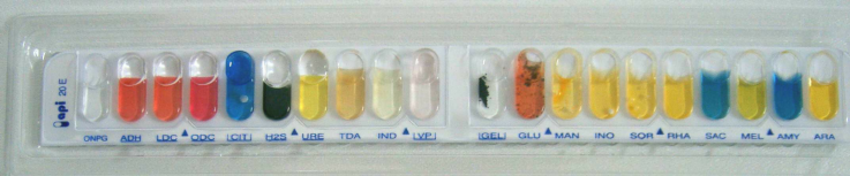
\includegraphics[width=1\textwidth]{image/Typical-Salmonella-reaction-of-API-20E-test-kit-After-incubation-in-a-humidity-chamber.png}
    \caption{Typical Salmonella reaction of API 20E test kit. After incubation in a humidity chamber for 18-24 hours at 37°C, the colour reactions were read (some with the aid of added reagents as supplied by the kit). The data were analysed by the manufacturer’s software and positive results with ≥ 89\% probabilities were confirmed as Salmonella .}
    \label{F-01}
\end{figure}
其中涉及到的生化反应如下表所示:
\begin{figure}[H]
    \centering
    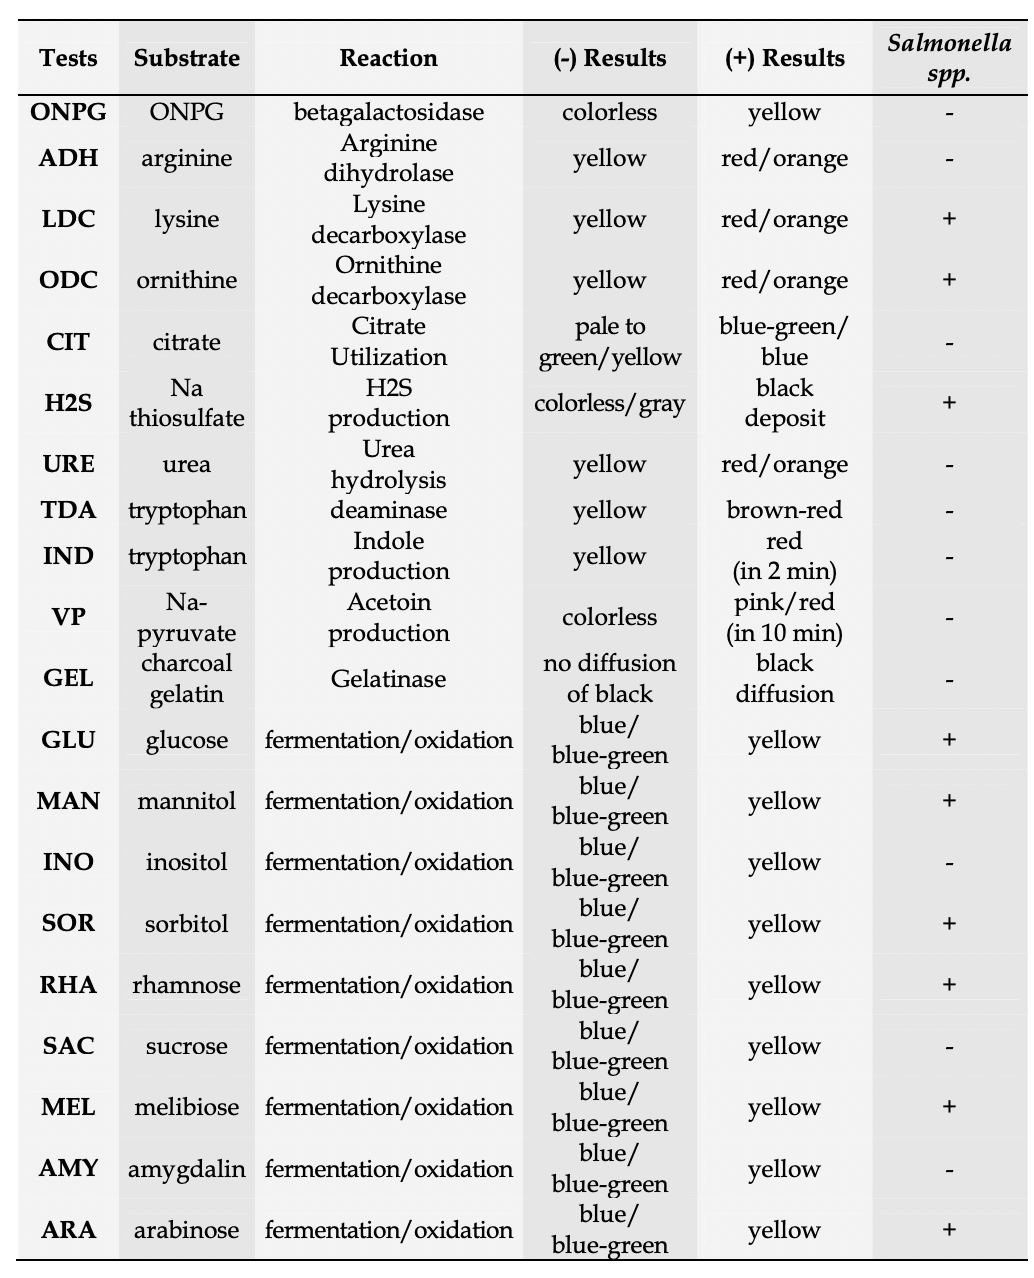
\includegraphics[width=0.5\textwidth]{image/Screen Shot 2021-05-10 at 10.48.35.png}
    \caption{ Biochemical reactions involved in API 20E (bioMérieux, Inc., France) test kits and typical \textit{Salmonella} reactions. }
    \label{F-02}
\end{figure}

\subsection{血清学分型}
\textbf{伤寒和副伤寒甲乙丙具有的抗原结构包括菌体抗原(O)、鞭毛抗原(H)及表面抗原。}
O抗原具有耐热性,
能耐受\SI{35}{\celsius} \SI{2.5}{\hour},它是分群的依据,其刺激机体产生的抗体以IgM为主,能够与相应的抗血清反应表现出颗粒状凝集;H抗原为不稳定的蛋白质抗原,
加热或用乙醇处理均会被破坏。沙门菌的H抗原有两个相,第一相特异性较高,在种间不同。
第二相为非特异相,为沙门菌属共有。
H抗原是定型的依据,其刺激机体产生的抗体以IgG为主,与相应的抗血清反应表现为絮状沉淀;表面抗原包括Vi、M和5抗原三种,Vi抗原不耐热,
加热\SI{60}{\celsius} \SI{0.5}{\hour}或经石炭酸处理即可破坏,
经人工培养基传代后也易失活。新分离的伤寒以及副伤寒丙沙门菌常带有此抗原,
它位于菌体的最表层,有抗吞噬及保护细菌免受相应抗体补体的溶菌作用,
当Vi抗原存在时可用于分型,但它也可阻止O抗原与相应抗体的凝集反应,必须在血清学鉴定时加以注意。\upcite{戚中田2014医学微生物学}

\begin{figure}[H]
    \centering
    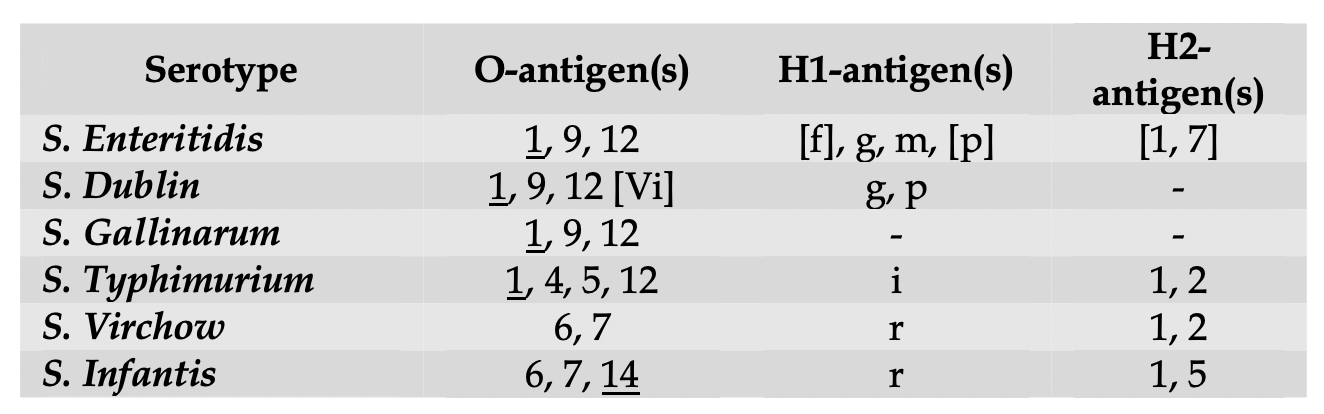
\includegraphics[width=0.7\textwidth]{image/Screen Shot 2021-05-10 at 10.55.32.png}
    \caption{Examples for the antigenic formulas of Salmonella enterica subsp. enterica serotypes according to Kaufmann-White scheme (Poppoff and Le Minor, 2001). }
    \label{F-03}
\end{figure}

\textbf{利用ViII型噬菌体可将伤寒杆菌分为约100个噬菌体型},对追踪传染源有帮助。

\section{常用的非免疫学鉴定方法(包括分子生物学方法)}



\begin{enumerate}
    \item 生化试剂盒,只能分辨至属,如API 20 系列的试剂盒。
    \item 血培养,粪便培养,尿培养,十二指肠引流液的培养,玫瑰疹刮取液的培养等,后续进行镜检。 (Sensitivity:~50\%, Specificity:~100\%)
    \item 不经培养直接进行PCR,例如PCR, nested, multiplex and real-time PCR等。(Sensitivity:~90\%, Specificity:~100\%)
\end{enumerate}

\section{常用的免疫学鉴定方法}

\begin{enumerate}
    \item 伤寒血清凝集试验(肥达反应, Widal reaction)所用的抗原有伤寒杆菌菌体(O)抗原,鞭毛(H)抗原、副伤寒甲、乙、丙鞭毛抗原5种。(Sensitivity:~65\%, Specificity:~90\%)
    \item TPTest (Sensitivity:~96\%, Specificity:~96\%)
    \item SD Bioline,Mega Salmonella,PanBio等,基于 ELISA 检测IgG,IgM,LPS等的存在。(Sensitivity与Specificity随厂商不一)
    \item Typhidot,LifeAssay Test-it,Tubex TF,基于dot blot的方法。(Sensitivity与Specificity随厂商不一)
\end{enumerate}

\section{Protocols}

具体试剂盒的Protocol见厂商给出的说明,下面只列举两个经典常用的流程,供参考。

\small
\subsection{血培养 Blood culture}

Blood samples were collected under aseptic precautions, 
5ml from children and 10ml from adults respectively and inoculated into Brain Heart Infusion Broth with SPS from HiMedia India.
Another 2 to 3ml blood was collected in sterile plain tube and allowed to clot till the serum separated. 
Serum was stored at \SI{-20}{\celsius} in small aliquots, properly labelled and used for both Widal test and Dot blot assay. 
Samples thus, collected were processed for microbiological examination using standard procedures.

Blood culture bottles were incubated aerobically at \SI{37}{\celsius}. 
Sub-cultures were made on Blood agar and MacConkey agar on every alternate day till the 7th day. 
The growth of Salmonella was identified as per standard protocol and confirmed by standard biochemical tests followed by 
sero-agglutination test using antisera. 
Antimicrobial susceptibility testing was done for all isolates using Kirby Bauer disc diffusion method.\cite{maheshwari2016comparative}

\subsection{肥达反应 The Widal test}

The Widal test was performed by tube method and it was considered positive when 
a titre of equal to or more than 160 was observed as the prevailing titre in the 
region was 120. Dot blot assay based on the principle of Enzyme Immuno Assay (EIA) was carried out and interpreted using Typhipoint (AB Diagnostics, India) as per manufacturer’s instructions.
\cite{maheshwari2016comparative}


\bibstyle{unsrt}
\bibliography{references}{}
\end{document}
